\documentclass[12pt, a4paper, twoside, romanian]{teza-upb}
\setcounter{secnumdepth}{3}
\setcounter{tocdepth}{3}
\usepackage{babel}
\usepackage{graphicx}
\usepackage{amsthm}
\usepackage{pbox}
\usepackage{amsfonts}
\usepackage{url}
\usepackage{minted}
\usepackage{fca}
\graphicspath{ {images/} }
\usepackage[
  bookmarksnumbered,
  bookmarks,
  bookmarksopen=true,
  pdftitle={Licenta Chereji Mihai},
  linktocpage
  ]{hyperref}

\singlespacing
\newtheorem{defn}{Definiție}
\newtheorem{example}{Exemplu}
\newtheorem{theorem}{Teoremă}

\begin{document}

\author{Mihai Chereji}

\title{Romagna: o abordare modernă asupra uneltelor de analiză conceptuală a datelor}


\facultatea{Facultatea de Electronică, Telecomunicații și Tehnologia Informației}
\tiplucrare{licență}
\domeniu{Calculatoare și tehnologia informației}
\catedra{Telecomunicații}
\program{Ingineria informației}
\titlulobtinut{Inginer}
\director{Christian Săcarea} 

\submissionmonth{Iulie} 
\submissionyear{2014} 

\beforepreface
\listoffigures
\listoftables
\abbreviations{ 
  FCA = Formal Concept Analysis (Analiza Conceptuală Formală)\\
  DOM = Document Object Model \\
  SVG = Scalable Vector Graphics (Grafice Scalabile Vectoriale)\\
  HTML = HyperText Markup Language (limbaj de marcaj hiper-textual)\\
  XML = eXtendable Markup Language (Limbaj extensibil de marcaj)\\
  SQL = Structured Query Language (Limbaj de Interogare Structurată)\\
  LLVM = Low Level Virtual Machine \\
  MVC = Model View Controller \\
}
\afterpreface 

\chapter*{Introducere}

  Big-data a devenit un domeniu foarte căutat în zilele noastre, devenit un cuvânt repetat de toată lumea, de la programatori la oameni de marketing. 
  Acest lucru se-ntâmplă deoarece lumea se \textit{înneacă} în date, adunate din diferite surse. Site-urile înregistrează fiecare mișcare a utilizatorilor, există pedometre care încarcă pe Internet numărul de pași făcut de utilizator în fiecare oră, datele de analiză medicală întorc tot mai multe date. 
  Interpretarea lor devine din ce în ce mai grea, și tendința este de a se folosi metode de \textit{machine learning}, ceea ce presupune învățarea automată (câteodată semi-automată) a calculatoarelor prin prelucrarea repetată a unei cantități imense de date.
  
  \textbf{Analiza conceptuală formală} oferă o alternativă, în care adunarea datelor este automată dar prelucrarea și interpretarea datelor este realizată de om, bazându-se pe câteva principii matematice bine definite și (relativ) ușor de înțeles. 

  Acest câmp a început în anii 80 la Universitatea din Darmstadt, ca o evoluție a teoriei clasice a laticelor. Între timp, s-a dezvoltat într-un câmp care adună tot mai mulți cercetători și își dovedește utilitatea practică dincolo de câmpul din care s-a tras și dincolo de matematica abstractă.

  Ce e mai spectaculos e că totul se bazează pe câteva idei simple, elegante, generale, frumoase am putea spune, încât duc aproape de \textit{filozofia platonică} (un concept este alăturarea unei mulțimi de obiecte descrise de unele proprietăți și mulțimea acelor proprietăți).

  Unele din cele mai utilizate rezultate ale acestei metode de analiză sunt laticele de concept, diagrame care reprezintă ierarhiile conceptelor descrise mai sus. 
  
  \begin{figure}[h!]
\begin{minipage}{.65\textwidth}
\unitlength 1.3mm
\begin{diagram}{40}{55}
\Node{1}{20}{10}
\Node{2}{35}{20}
\Node{3}{5}{30}
\Node{4}{35}{40}
\Node{5}{20}{50}
\Edge{1}{2}
\Edge{1}{3}
\Edge{2}{4}
\Edge{3}{5}
\Edge{4}{5}
\Numbers
\leftAttbox{3}{2}{2}{1.}
\rightAttbox{2}{2}{2}{disqualified}
\rightAttbox{4}{2}{2}{2.}
\leftObjbox{3}{2}{2}{Hamilton}
\rightObjbox{2}{2}{2}{Massa}
\rightObjbox{4}{2}{2}{Alonso}
\end{diagram}
\end{minipage}
\caption{Exemplu de latice de concepte}
\end{figure}

  Se observă că dincolo de utilitatea practică (descrisă în capitolele ce urmează), laticea este \textit{frumoasă}. Fără a încerca să-i descifreze înțelesul, oricine poate observa că este unul din acele produse ale științei care, ne-intenționat, poate fascina și studenții artelor.

  Cu toate acestea, domeniul FCA duce lipsă de unelte frumoase (vom explica, în capitolele ce urmează ce înțelegem prin \textit{software frumos}), chiar dacă există tot mai multe programe care doresc să ajute cercetătorii în acest domeniu. Unele frustrează încă de la încercarea procesului de instalare, altele mistifică cercetătorul prin mesaje de eroare criptice, iar altele, poate, doar se mișcă prea încet, sau sunt prea greu de folosit.

  În cele ce urmează dorim să descriem pe scurt domeniul analizei conceptuale formale (în capitolul \ref{chapter:1}), starea soft-ului existent acum (în capitolul \ref{chapter:2}), și o nouă aplicație (capitolul \ref{chapter:3}), care dorește să rezolve unele din problemele întâlnite de oamenii interesați în acest domeniu, și poate, să atragă prin software bine gândit (și, sperăm, \textit{bine realizat}, căci un concept fără nici un obiect nu are cuprins - \textit{veți înțelege după ce veți parcurge primul capitol}) adepți noi.

\chapter{Analiza conceptuală formală}
\label{chapter:1}
  \section{Introducere}
    Analiza conceptuală formală este o metodă de sistematizare a datelor în \textbf{concepte}, definite la modul larg ca tupluri constituite din mulțimi de obiecte care împărtășesc anumite atribute și mulțimea acelor atribute. Este o reinterpretare a teoriei clasică a laticelor, dezvoltată în principal în anii '30, axată către partea practică. Conceptul a fost introdus în lucrarea seminală a lui Robert Wille din 1982 \cite{wille:1982}, iar termenul a fost introdus în 1984 de același autor. În ultimele decenii, domeniul a atras multe contribuții și și-a dovedit utilitatea în domenii cum ar fi analiza și vizualizarea datelor, managementul informației.
  \section{Concepte matematice de bază}
    Pentru a avea o mai bună înțelegere a conceptelor pe care se bazează aplicația, vom explica pe scurt definițiile de bază ale domeniului.
    \subsection{Mulțimi ordonate, latice, latice complete}
    Vom începe cu câteva concepte elementare de algebră a mulțimilor, deoarece acest domeniu se bazează în întregime pe ele.
    \begin{defn}
      O mulțime $M$ este ordonată dacă se poate aplica asupra sa o relație $R$ care îndeplinește următoarele condiții:
      \begin{description}
        \item [Reflexivitate] $xRx$
        \item [Antisimetrie] $xRy, x \neq y \Rightarrow yRx$ e fals
        \item [Tranzitivitate] $xRy, yRz \Rightarrow xRz$
      \end{description}
      $\forall x, y,z \in M$. Relația $R$ se numește o \textbf{relație de ordine}.
    \end{defn}

    Cel mai simplu exemplu, intuitiv exemplu este mulțimea numerelor reale $ \mathbb{R}$, alături de relația $\le$. Notăm o mulțime ordonată cu relația $\le$ cu $(M, \le)$.

    \begin{defn}
      Un element $y$ al mulțimii $M$ este \textbf{vecinul superior} al lui $x$ dacă $x < y$ și nu există nici un $z$ astfel încât $x < z < y$. În mod invers, $x$ este \textbf{vecinul inferior} al lui $y$.
    \end{defn}

    Putem nota relația de vecinătate astfel: $x \prec y, y \succ x$.

    \begin{defn}
      Două elemente ale unei mulțimi ordonate sunt \textbf{comparabile} dacă $x \le y$ sau $y \le x$ (adică relația $\le$ se aplică asupra lor). Altfel sunt \textbf{incomparabile}. Un \textbf{lanț} este o submulțime în care oricare două elemente sunt comparabile. Un \textbf{anti-lanț} este o submulțime în care oricare două elemente sunt incomparabile.
    \end{defn}

    \begin{defn}
      Fie $(M, \le)$ o mulțime ordonată, și $N$ o submulțime a sa. Înțelegem prin \textbf{minorantul} mulțimii $N$ un element $i$ astfel încât $\forall a \in N, i \le a$. În mod invers, \textbf{majorantul} mulțimii $s$ este definit prin $\forall a \in N, s \ge a$.
      Putem nota mulțimea tuturor minoranților a grupului $N$ cu $I$. Elementul cel mai mare din această mulțime este numit \textbf{infimumul} mulțimii $N$. Invers, cel mai mic element din mulțimea majoranților este numit \textbf{supremumul} mulțimii $N$.
    \end{defn}

    Minorantul se poate nota cu $\wedge N$ sau $\inf N$, iar supremumul cu $\vee N$ sau $\sup N$.

    \begin{defn}
      O mulțime ordonată $M$ este numită o \textbf{latice} dacă $\forall x,y \in M, \exists x \vee y, \exists x \wedge y$. În alte cuvinte, o mulțime ordonată este o latice dacă pentru orice 2 elemente ale mulțimii există supremum și infimum. O latice este \textbf{completă} dacă pentru orice submulțime (finită) a ei există supremum și infimum.
    \end{defn}

    Orice latice completă are un element superior, numit \textbf{elementul unitate}, și un element inferior, numit \textbf{elementul zero}.

    \begin{defn}
      Conform \cite{Carpineto:2004:CDA:975252} O \textbf{conexiune Galois} este compusă din două mulțimi ordonate, $M, N$ și două funcții $\gamma, \psi$ astfel ca $ \gamma: M \rightarrow N, \psi : N \rightarrow M$, dacă și numai dacă:
    \begin{enumerate}
      \item $m_1 \le m_2 \Rightarrow  \gamma m_1 \ge \gamma m_2$
      \item $n_1 \le n_2 \Rightarrow \psi n_1 \ge \psi m_2$
      \item $m \le \psi \gamma m,  n \le \gamma\psi n $
    \end{enumerate}
    sau, echivalent, $m \le \psi n \Leftrightarrow n \le \gamma m$
    \end{defn}

    \subsection{Context, concept, ierarhie de concepte}
    \begin{defn}
      În cadrul analizei conceptuale, un \textbf{context} $K = (G, M, I)$ este format din 2 mulțimi, $G$ și $M$, și o relație binară $I$ între acestea. Mulțimea $G$ reprezintă obiecte, iar $M$ atribute.
    \end{defn}

      Literele provin din limba germană, în care conceptele au fost descrise inițial, de la Gegenstände și MerKmale, respectiv. Relația $I$ e numită \textbf{relația de incidență}, iar $gIm$ poate fi citit ca ``obiectul $g$ este descris de atributul $m$'', sau ``atributul $m$ descrie obiectul $g$''.

      \begin{example}
      Preluăm următorul exemplu din \cite{Carpineto:2004:CDA:975252}, un context (foarte redus)al animalelor vertebrate.
        \begin{table}[h]
          \begin{tabular}[c]{| c | c | c | c | c | c | c | c | c | c | c |}
            \hline
            \multicolumn{2}{|c|}{} &
            \parbox{1.2cm}{\centering respiră în apă\\(a)} &
            \parbox{1.2cm}{\centering zboară \\(b)}         &
            \parbox{1.2cm}{\centering  are cioc\\(c)}       &
            \parbox{1.2cm}{\centering  are mâini \\(d)}      &
            \parbox{1.2cm}{\centering  are schelet \\(e)}     &
            \parbox{1.2cm}{\centering are aripi \\(f)}       &
            \parbox{1.2cm}{\centering  trăiește în apă\\(g)}  &
            \parbox{1.2cm}{\centering naște pui vii \\ (h)}  &
            \parbox{1.2cm}{\centering  produce lumină \\(i)} \\ \hline
              1 & Liliac        &   & $\times$ &   &   & $\times$ & $\times$ &   & $\times$ &     \\
              2 & Vultur        &   & $\times$ & $\times$ &   & $\times$ & $\times$ &   &   &     \\
              3 & Maimuță       &   &   &   & $\times$ & $\times$ &   &   & $\times$ &     \\
              4 & Pește papagal & $\times$ &   & $\times$ &   & $\times$ &   & $\times$ &   &     \\
              5 & Pinguin       &   &   & $\times$ &   & $\times$ & $\times$ & $\times$ &   &     \\
              6 & Rechin        & $\times$ &   &   &   & $\times$ &   & $\times$ &   &     \\
              7 & Pește lanternă& $\times$ &   &   &   & $\times$ &   & $\times$ &   &  $\times$  \\
            \hline
            \end{tabular}
          \caption{Un context al animalelor vertebrate. Sursa: CDA \cite{Carpineto:2004:CDA:975252}}
          \label{table:animale-vertebrate}
        \end{table}
      \end{example}

    Pentru $A \subseteq G$, definim
    $ A' = \{m \in M | gIm, \forall g \in A\} $.

    În mod asemănător, pentru $B \subseteq M$, $B' = \{g \in G | gIm, \forall m \in B \}$.

    În cuvinte, $A'$ este mulțimea tuturor atributelor (din contextul la care ne raportăm) care descriu toate obiectele din $A$.

    \begin{defn}
      Un \textbf{concept} al contextului $(G, M, I)$ este definit de $A \subseteq G$, $B \subseteq M$, unde $A' = B$ și $B' = A$.
    \end{defn}

    În engleză, mulțimea $A$ (a tuturor obiecte descrise de atributele conceptului) este numită \textbf{extent} (cuprins), iar $B$ (atributele care descriu toate obiectele conceptului) \textbf{intent}(conținut).


Fie $(G, M, I)$ un context, și $A, A_1, A_2$ submulțimi ale lui $G$, iar $B, B_1, B_2$ submulțimi de-ale lui $M$. Conform \cite{Ganter:1997:FCA:550737}, atunci:

    \begin{enumerate}
        \item $A_1 \subseteq A_2 \Rightarrow A^{'}_{1} \supseteq A^{'}_2$
        \item $A  \subseteq A'''$
        \item $A' = A'''$
        \item $A \subseteq B' \Longleftrightarrow B \subseteq A' \Longleftrightarrow A \times B \subseteq I$
    \end{enumerate}

    Proprietăți echivalente se observă imediat și pentru $B, B_1, B_2$.

    Având în vedere că $ ': \mathcal P \left(G \right) \rightarrow \mathcal P \left(M\right)$ și $B' : M \rightarrow G$, cei doi operatori pot fi combinați pentru a crea $A''$ și $G''$, care au ca domeniu mulțimea submulțimilor $G$ și $M$ respectiv. 

Se observă pornind de la proprietățile enumerate mai sus că cele două funcții de derivare descriu o conexiune Galois între mulțimile submulțimilor pentru obiecte ($\mathcal P \left(G \right)$) și ($\mathcal P \left( M \right) $)

În exemplul de mai sus, $\{2, 4\}'' = \{2, 4, 5\}$, $\{d, h\}'' = \{d, e, h \}$.


  Câteva proprietăți de remarcat ale conceptelor, așa cum sunt definite:
  \begin{itemize}
        \item Nu orice submulțime de obiecte definește cuprinsul unui concept. Din cele descrise mai sus, rezultă că e necesar ca $ A = A''$ pentru $A$ să fie cuprinsul unui concept.

        Ca exemplu, în tabelul \ref{table:animale-vertebrate}, $\{6\}$ nu definește un concept, deoarece $\{6\}'' = \{4, 6, 7\}$, adică toate atributele care descriu rechinul în contextul nostru descriu de-asemenea și peștele lanternă, și peștele papagal.
        \item Intersecția oricâtor cuprinsuri (sau conținuturi) de concepte are ca rezultat întotdeauna un alt cuprins (respectiv conținut).
        \item În urma reuniunii lor, pe de altă parte, rareori rezultă un alt cuprins.
        \item Mulțimea conceptelor unui context este o mulțime ordonată, dacă definim o relație de ordine în felul următor:
          \begin{defn}
            Fie $(A_1, B_1)$ și $(A_2, B_2)$ concepte ale contextului $K = (G, M, I)$. Spunem că $(A_2, B_2)$ este un \textbf{subconcept} al lui $(A_1, B_1)$ (notat $(A_2, B_2) \le (A_1, B_1)$ dacă $A_2 \subseteq A_1$. Astfel, $(A_1, B_1)$ este \textbf{supraconceptul} lui $(A_2, B_2)$
          \end{defn}
  \end{itemize}

    \begin{theorem}
      \textbf{Teorema de bază a laticelor de concepte} - 
      Fie un context $(G, M, I)$, și o mulțime ordonată $\mathcal C \left(G, M, I; \le \right)$ se numește laticea de concepte a contextului, care are supremumul și infimumul descrise de:
      $$ \bigwedge_{t \in T}(A_t, B_t) = \left( \bigcap_{t \in T} A_t, \left( \bigcup_{t \in T} B_t \right)'' \right)$$
      $$ \bigvee_{t \in T} (A_t, B_t) = \left( \left( \bigcup_{t \in T} A_t \right)'', \bigcap_{ t \in T} B_t \right)$$
    \end{theorem}

  

    \begin{itemize}
      \item Diagrame Hasse
      \item Reducerea și clarificarea contextelor
      \item Rezolvarea contextelor cu valori multiple
    \end{itemize}

  \section{Algoritmi relevați}

  \section{Utilizări practice}
  \label{sec:utilizari-practice}
%\begin{cxt}
%\cxtName{Formula 1}
%\att{1.}
%\att{2.}
%\atr{disqualified}
%\obj{x..}{Hamilton}
%\obj{.x.}{Alonso}
%\obj{.xx}{Massa}
%\end{cxt}

\chapter{Starea actuală}
\label{chapter:2}

  În clipa de față există multe programe folosite pentru diferite aspecte ale analizei conceptuale formale. O listă mai dezvoltată, care adună majoritatea programelor disponibile poate fi găsită la \cite{utapriss:software}.

  Mai jos vom discuta doar câteva programe care au influențat dezvoltarea Romagnei, sau sunt relevante din motive istorice, arhitecturale, etc.
  \section{Navigatoare de concepte}
    \subsection{Toscana}
      Toscana\cite{Vogt:1995:Toscana} a fost lansat în 1995, și a fost unul din cele mai folosite unelte de explorare a laticelor de concepte pe parcursul următorilor ani.

      Toscana este astăzi probabil cel mai bine ținută minte ca precursorul programului ToscanaJ, folosit și astăzi, prezentat în detaliu mai jos (\ref{subsec:toscanaj}).

      În ciuda eforturilor noastre, unealta nu a fost găsită pentru descărcare.

    \subsection{Toscanaj}
    \label{subsec:toscanaj}
      ToscanaJ(\cite{Toscanaj:homepage}) este ``moștenitorul direct'' al lui Toscana, lucru evidențiat și de nume (J-ul vine de la Java).

      După cum spune chiar site-ul programului \cite{Toscanaj:toscanaj}: ``E o unealtă de vizualizare pentru scheme conceptuale foarte avansată, care reușește să afișeze informație interogată dintr-o bază de date în diagrame de latice, sau direct din structuri de date luate din memorie.''
      \subsubsection{Funcționalități}
      \label{subsubsec:toscanaj-functionalitati}
      
        Din nou, citând site-ul programului\cite{Toscanaj:toscanaj}, prezentăm câteva funcționalități ale programului:

        \begin{quote}
          ``
          \begin{itemize}
            \item Afișarea diagramelor simple și imbricate.
            \item Culoarea unui nod reprezintă mărimea contingentului obiectelor (poate fi modificat să reprezinte cuprinsul), deasemenea mărimea nodului poate fi folosită pentru același tip de informație.
            \item Mulțimea de obiecte de interes poate fi filtrată printr-un dublu click asupra nodurilor
            \item Nodurile din diagramă pot fi selectate pentru a fi scoase în evidență, pentru a ajuta citirea \textit{[n.t. diagramei]}.
            \item Diagramele pot fi exportate ca SVG, PNG și JPEG. Informații adiționale despre cum diagrama a fost obținută sunt exportate ca fișiere text separate, prin memoria temporară a calculatorului \textit{(clipboard)}, sau direct în fișierul SVG (ca elementul \verb=<desc>=).
            \item Etichetele nodurilor pot avea conținut diferit, folosindu-se de fragmentele de SQL specifice datelor
            \item Vizualizări adiționale a bazei de date pot fi deschise din diagramă, de exemplu folosind șabloane HTML în care rezultatele interogărilor sunt afișate.
            \item Interfața de vizualizare a bazei de date a fost gândită ca o interfață pentru pluginuri pentru a ușura extinderea ToscanaJ pentru scopuri specifice.
            \item Descrieri HTML pot fi atașate schemei, diagramelor și atributelor
            \item Vederile bazelor de date pot fi folosite pentru atribute, de exemplu pentru a interoga un URL din baza de date care e mai apoi deschis într-un navigator extern.
          \end{itemize}
          ''
        \end{quote}

        Având în vedere că scopul programului Romagna este de a oferi o alternativă programului Toscana(J), aceste funcționalități se vor regăsi și în Romagna, alături de altele, descrise în capitolul \ref{sec:rationament}.

        Mai jos prezentăm două capturi de ecran care prezintă programul ToscanaJ.

        \begin{figure}[h]
          \centering
          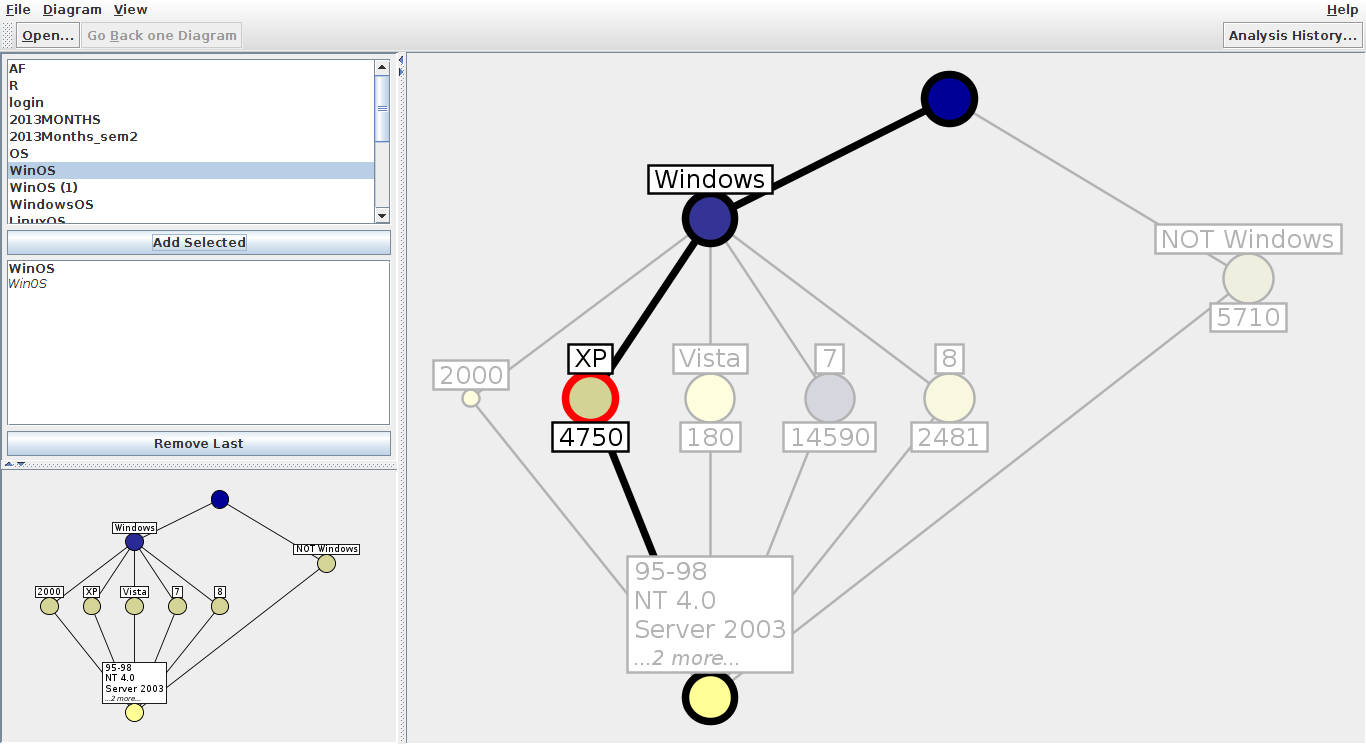
\includegraphics[width=\textwidth, natwidth=1366, natheight=744]{toscanaj-1.png} \\ 
          \caption{ToscanaJ, afișând o latice simplă generată din date de acces ale unui site web}
          \label{screenshot:toscana-1}
        \end{figure}
        \begin{figure}[h]
          \centering
          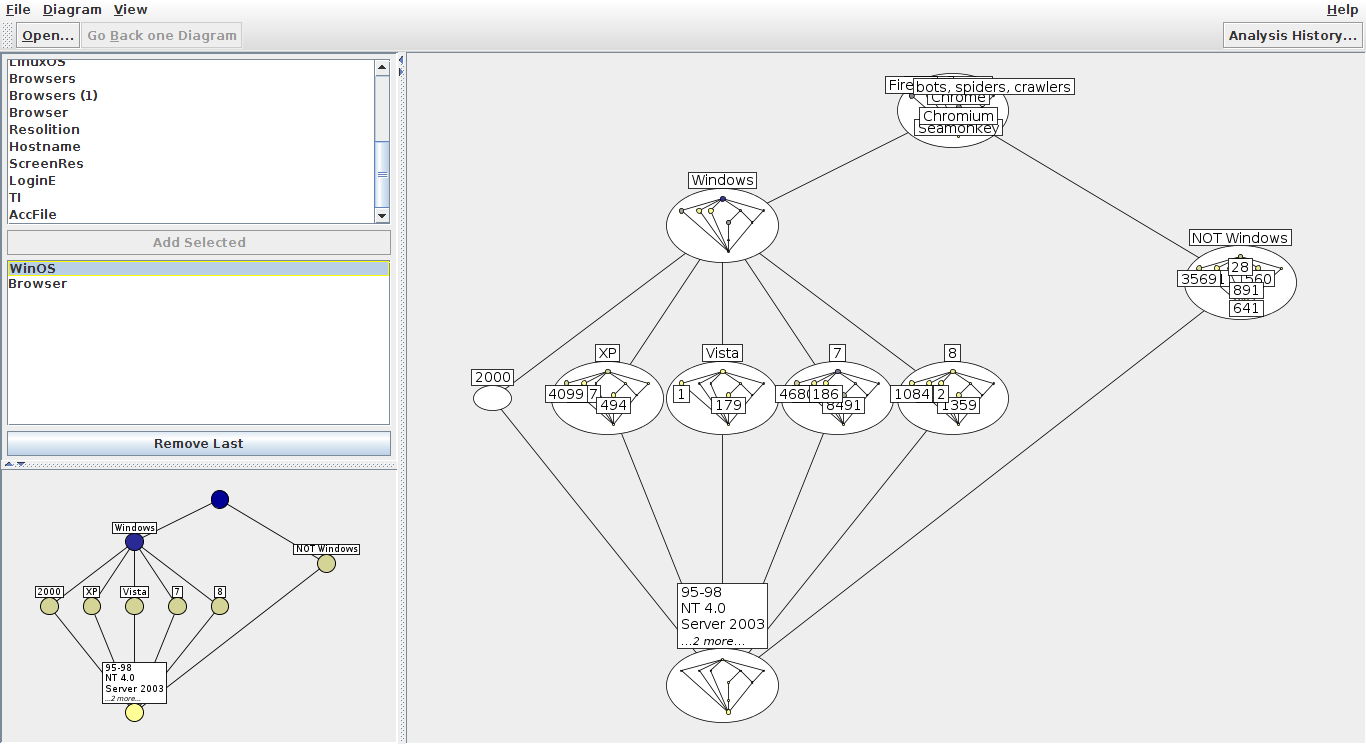
\includegraphics[width=\textwidth, natwidth=1366, natheight=744]{toscanaj-2.png}
          \caption{ToscanaJ, afișând aceeași latice ca în \ref{screenshot:toscana-1}, de data aceasta imbricată cu altă diagramă}
          \label{screenshot:toscana-2}
        \end{figure}

        Interfața ToscanaJ este punctul de pornire pentru Romagna. Vom încerca să păstrăm anumite elemente comune, pentru a ajuta utilizatorii obișnuiți, dar vom face, bine-nțeles schimbări și adaptări, mai ales luând în considerare diferențele convențiilor dintre interfețele aplicațiilor web, și cele desktop.

        ToscanaJ este, asemenea Romagna, doar un navigator de concepte. Modelarea conceptelor din date este realizată cu ajutorul altor programe din suita din care face parte și ToscanaJ.

        \begin{description}
            \item[Elba] este un editor pentru schemele conceptuale, legat de baze de date.
            \item[Siena] este un editor pentru scheme conceptuale, foarte asemănător cu \textbf{Elba}, diferența fiind că Siena nu are nevoie de o legătură cu o bază de date, putând descrie concepte simple direct în program.
        \end{description}

  \subsection{GaloisExplorer}
    GaloisExplorer \cite{GaloisExplorer:homepage} este un program mai recent, cu ultima actualizare în 2009.

    Are o intefață realizată în QT, ceea ce îi permite să funcționeze pe mai multe platforme. O abordare interesantă, dar în cele din urmă doar cu valoare estetică, este prezentarea laticelor în 3d (\ref{screenshot:galoisexplorer}).
   
    Din păcate, folosește anumite librării 3d (coin3d\cite{Coin:homepage}) care nu sunt imediat disponibile și care necesită compilare manuală.

    Pentru mulți utilizatori care nu au cunoștințe avansate de calculatore, aceste impedimente sunt motiv suficient pentru a abandona această instalare.
    \begin{figure}[h]
      \centering
      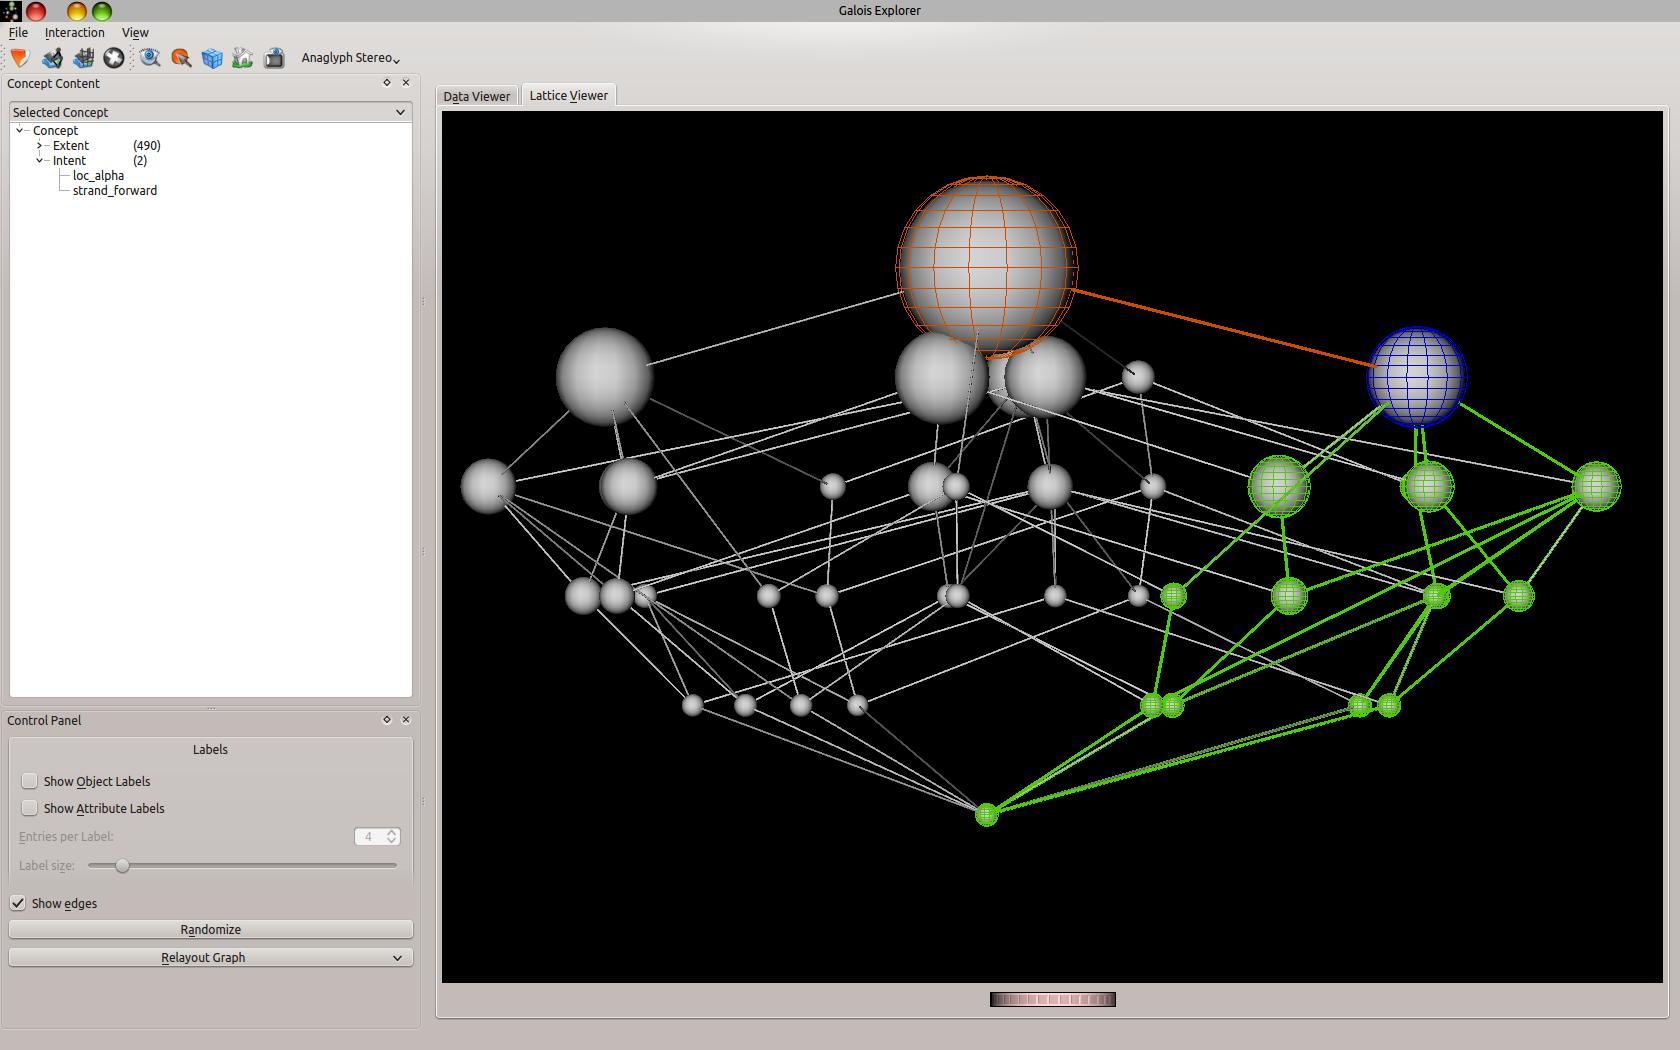
\includegraphics[width=\textwidth]{GaloisExplorer_latticeView}
      \caption{GaloisExplorer, afișând o diagramă în 3d. Sursa: site-ul proiectului \cite{GaloisExplorer:sourceforge}}
      \label{screenshot:galoisexplorer}
    \end{figure}

  \section{Software conex}
  %TODO: define Duquenne-Guiges
  %TODO: schimbă traducerile trimise de prof

    În această secțiune vom prezenta câteva alte programe remarcabile în domeniul FCA, sau care au avut un impact indirect asupra dezvoltării Romagna:
    \begin{description}
      \item[FCAStone] dezvoltat de Uta Priss, e un program care urmărește obținerea inter-operabilității între diferite programe pentru FCA (numele vine de la Piatra \textit{[n.t. Stone = Piatră]} Rosetta). Astfel, convertește fișierele folosite de mai multe suite în FCA. Pe lângă asta, convertește contexte în latice de concepte, și latice de concepte în formate grafice (atât vectoriale cât și raster).
      \item[Conexp] dezvoltat de Serhiy A. Yevtushenko, este o unealtă scrisă în Java, folosită în principal în scopuri educaționale (dar nu numai), are numeroase funcționalități de modelare a contextelor, dintre care amintim (preluate de site-ul programului \cite{conexp:users}):
        \begin{itemize}
            \item calculează numărul de concepte formale dintr-un context dat
            \item calculează laticea de concepte
            \item permite explorarea atributelor
            \item calculează mulțimea de implicații Duquenne-Guiges
            \item calculează regulile de asociații
        \end{itemize}
      \item[conexp-clj] O reimplementare scrisă de Daniel Borchmann în limbajul de programare Clojure a programului de mai sus. Programul pune accentul pe linia de comandă și programarea interactivă în domeniul FCA.
      \item[OpenFCA] Este o suită de trei aplicații, din care Conflexplore este o aplicație bazată pe Flex, folosită pentru explorarea conceptelor, atât tabelar cât și printr-o formă simplă de latice de concepte.  
      \item[\LaTeX for FCA] \cite{LatexForFCA:homepage} Plugin pentru \LaTeX, scris de Bernhard Ganter, oferă câteva ``environment''-uri noi, folosite și în această lucrare, care permite aranjarea ușoară în pagina a contextelor și a laticilor derivate din acestea.
    \end{description}

\chapter{Romagna}
\label{chapter:3}

  Romagna este o aplicație dezvoltată începând cu anul 2014, pornită la Universitatea Babeș-Bolyai ca o alternativă folosindu-se de tehnologiile web pentru un navigator de concepte modern.

  Numele (Romagna) este o referință directă suitei de programe care a inspirat această aplicație, Toscana. Romagna este o regiune istorică a Italiei aflată la nordul Toscanei. 

  Pe lângă funcționalitățile ale aplicației ToscanaJ descrise în sub-subsecțiunea \ref{subsubsec:toscanaj-functionalitati}, Romagna are câteva funcționalități noi plănuite.

  Dezvoltarea acestei aplicații are câteva scopuri \textit{(diferite de funcționalități)} principale, prezentate în secțiunea următoare.

  \section{Raționament}
  \label{sec:rationament}

    \subsection{Ușurință de utilizare}
    \label{subsec:usurinta-de-utilizare}
      Uneltele destinate FCA trebuie gândite ca programe pentru consumatori, utilizatori obișnuiți. Publicul țintă al acestor aplicații nu sunt neapărat programatori sau oameni cu experiență în folosirea avansată a calculatoarelor. Oamenii care beneficiază cel mai mult de asemenea aplicații sunt cercetători în domenii foarte diferite (după cum se vede în secțiunea de aplicații practice \ref{sec:utilizari-practice})

      Din acest punct de vedere, este părerea autorului că soft-ul existent în acest domeniu nu satisface necesitățile publicului său țintă. 

      Pentru clarificare, următoarele puncte trebuie îndeplinite pentru a considera o aplicație ușor de folosit:
      \begin{itemize}
      \item Aplicația trebuie să fie \textbf{ușor de instalat}. Programatorii de multe ori scapă din vedere acest aspect, dacă nu e vorba de un produs comercial, care are nevoie de cât mai mulți utilizatori.
        E inadmisibil să se ceară compilarea manuală a unei librării C++, sau instalarea unui server MySQL unui utilizator obișnuit pentru a utiliza un program. Romagna, fiind o aplicație web, sare peste acești pași. Singurii pași pre-mergători folosirii aplicației sunt pregătirea datelor pentru consum de către aplicație și familiarizarea cu interfața aplicației.
      \item Aplicația trebuie să fie \textbf{disponibilă pe mai multe platforme}. Utilizatorii nu vor instala un alt sistem de operare pentru a testa o aplicație. 
        În schimb, majoritatea utilizatorilor au la dispoziție un navigator web modern, cum ar fi Mozilla Firefox, Google Chrome, etc. 
        Aceste medii de aplicații (pentru că navigatoarele web și mediul de execuție al limbajului JavaScript pus la dispoziție de acestea a devenit un mediu de aplicații) se actualizează automat, permițând utilizarea celor mai noi funcționalități unei majorități a utilizatorilor acestora.
        \item Aplicația trebuie să ofere \textbf{date de ieșire utile} utilizatorului. Ne referim aici bine-nțeles la rezultatele așteptate de utilizator, prezentate într-un mod clar, dar și la mesajele de erori, care trebuie să fie inteligibile, să ofere cursuri de acțiune care să rezolve problema întâmpinată, într-un limbaj non-tehnic, pe cât posibil.
          Erorile criptice, cum ar fi stack-trace-uri, sau excepții afișate pe ecran descurajează utilizatorul obișnuit.
        \item Aplicația trebuie să aibă \textbf{o interfață plăcută}. E părerea autorului că, deși utilizabile, interfețele generate de aplicații Java în general oferă o experiență neplăcută, nu se integrează în stilul sistemului de operare. Aplicațiile web sunt mult mai ușor de estetizat, mai ales cu ajutorul unor framework-uri CSS, dintre care amintim Twitter Bootsrap sau Zurb Foundation.
          \item Ca o ultimă alternativă, aplicația trebuie să vină \textbf{însoțită de documentație}. Aceasta trebuie formulată într-un limbaj non-tehnic pentru utilizatori. 
          \item Opțional, aplicația ar trebui să aibă \textbf{interfața localizată}. Nu toți utilizatorii de calculatoare sunt vorbitori de engleză. Folosirea pictogramelor pentru realizarea interfeței poate ajuta, dar inclusiv în acest caz, diferențele culturale, sau conceptele prea complexe pe care dezvoltatorii încearcă să le transmită, pot descuraja utilizarea aplicației mai mult decât să ajute.
      \end{itemize}

      Romagna îndeplinește unele din condițiile de mai sus(ușor de instalat, ușor de găsit) prin natura aplicațiilor web, iar celelalte condiții constituie obiectul efortului autorului.

    \subsection{Folosirea web-ului, păstrarea confidențialității datelor}
    \label{subsec:confidentiality}

      Este o stare de fapt că în domeniul analizei datelor, integritatea și confidențialitatea acestora este o grijă constantă.

      Mulți cercetători lucrează de asemenea cu date care sunt, legal vorbind, secrete. Se înțelege astfel, că majoritatea potențialilor utilizatori \textbf{nu} vor avea încredere să trimită datele unui serviciu extern.

      Din aceste considerente, o arhitectură server peste web (și oferirea Romagnei ca serviciu) a fost imediat desconsiderată. Dar, cum am menționat în subsecțiunea \ref{subsec:usurinta-de-utilizare}, ușurința de utilizare este o altă calitate pe care încercăm să o regăsim în Romagna. 
      
      S-a ajuns astfel la compromisul (temporar) de a realiza \textbf{totul} în browser. Asta înseamnă accesarea datelor SQL în browser, prin tehnologii descrise în secțiunea \ref{sec:tehnologii}.

  \section{Tehnologii}
  \label{sec:tehnlogii}

    După cum am menționat, Romagna se bazează pe tehnologii web. Vom continua prin a descrie sumar principalele librării/framework-uri folosite și un raționament scurt pentru existența lor în proiect.

    \subsection{CoffeeScript}
      Unul din principalele motive pentru care browser-ul nu a fost mult timp acceptat ca o platformă matură pentru aplicații era absența altor limbaje de programare disponibile înafară de JavaScript.

      Această stare de fapt se schimbă încet din mai multe motive:
      \begin{itemize}
        \item JavaScript a evoluat și este considerat un limbaj de programare mai matur decât în perioada în care a fost scris ToscanaJ.
        \item Existența \textbf{emscripten}, descris pe scurt în subsecțiunea \ref{subsec:emscripten} și rezultatele obținute de acesta.
        \item Existența limbajelor care compilează \textit{în} JavaScript.
      \end{itemize}

      Unul din aceste limbaje este \textbf{CoffeeScript} \cite{ashkenas:2012:coffescript}. CoffeeScript nu introduce decât două concepte (clase versus prototipuri și array comprehensions) noi față de JavaScript, dar simplifică dezvoltarea prin câteva îmbunătățiri:
      \begin{itemize}
        \item Evitarea variabilelor globale
        \item Câteva scurtături de sintaxă (\verb=->= pentru a declara o funcție, \verb~=>~ pentru a declara o funcție legată de contextul actual, etc.) 
        \item Clarificarea operatorilor de comparație (\verb~==~ în CoffeeScript devine automat \verb~===~ în JavaScript, scăpând automat de o întreagă clase de erori).
      \end{itemize}
          Alături de sintaxa mai prietenoasă (o opinie personală a autorului), prin elidarea acoladelor în favoarea indentării pentru definirea blocurilor, am ales CoffeeScript ca limbajul principal pentru Romagna.

    \subsection{Ember.js}
      Ember.js este un framework scris în JavaScript, inspirat de Cocoa, și are ca scop ușurarea dezvoltării aplicațiilor web complexe, prin oferirea unui cadru MVC, cu o structură relativ rigidă. 
      
      Inițial aplicația nu era bazată pe niciun framework. Pe măsură ce complexitatea structurii a crescut, am realizat că recreem, involuntar, un sistem MVC, mai mult ca sigur imperfect.
     
      Am hotărât să reorganizăm codul în urma unei deliberări, bazându-ne pe faptul că un framework folosit de mii de oameni, cu teste funcționale și modulare la zi poate oferi o fundație puternică, fără a ne cheltui timpul ``re-inventând roata''. Din variantele disponibile de framework-uri pentru JavaScript, am ales Ember.js deoarece:
      \begin{itemize}
        \item Structura impusă se potrivește cu necesitățile proiectului.
        \item Posibilitatea schimbării ușoare a adaptorului a repozitoriului de date inclus în framework înseamnă că vom putea crea o variantă viitoare a Romagna care se includă comunicarea cu un server, funcționalitate care este plănuită pentru versiuni care vor urma.
        \item Funcționalitatea componentei \verb=Router=, care permite crearea de URL-uri, care pot fi salvate de utilizator, în funcție de navigarea sa prin aplicație, înseamnă că avem la îndemână o formă simplă de serializare și salvare a stării aplicației.
      \end{itemize}
    \subsection{d3.js}
      D3 (provenit din \textit{Data-Driven Documents} - Documente Bazate pe Date) este o librărie scrisă în JavaScript pentru manipularea DOM-ului relaționând cu date legate de elemente din document. Citând din abstractul lucrării \cite{bostock:2011:d3}:
      \begin{quote}
        ``Cu D3, designerii leagă în mod selectiv date de intrare de elemente arbitrare ale documentului, aplicând transformări dinamice pentru a genera, cât și a modifica conținut.''
      \end{quote}
      Devine clar din descrierea de mai sus că această librărie va ușura dezvoltarea aplicației, datorită posibilității de a lega \textit{conceptele} de reprezentarea acestora într-un mod care să permită modificarea acestei reprezentări în funcție de explorarea diagramelor de către utilizator, ceea ce, este, până la urmă scopul aplicației.
      \subsubsection{svg}
        D3 se bazează pe manipularea DOM-ului pentru a obține vizualizări dinamice de date. Deși HTML-ul poate fi stilizat, formele complexe și imaginile vectoriale sunt descrise în browser prin SVG \cite{Ferraiolo:01:SVG}, un standard de grafică vectorială vazată pe XML. Deși ajută la crearea unor aplicații de vizualizare complexe, SVG-ul vine cu problemele sale, care sunt descrise mai pe larg în sub-subsecțiunea \ref{subsubsec:svg-problems}.
    \subsection{sql.js}
      După cum am descris în secțiunea \ref{subsec:confidentiality}, pilonii pe care am decis să construim Romagna (ușurința de utilizare și păstrarea locală a datelor) pun în dificultate folosirea unei arhitecturi client-server, deoarece vrem un proces de instalare și folosire cât mai simplu (nici un proces de instalare nu e mai simplu decât deschiderea unei pagini web), iar utilizatorii nu-și vor trimite datele unei părți terțe, din temeri proprii sau pentru că nu au acest drept, lucrând cu date confidențiale.

      Astfel, compromisul este de a analiza SQL în browser, cu ajutorul sql.js \cite{sqljs:homepage}, care este defapt SQLite re-compilat în JavaScript cu ajutorul emscripten.

      SQL.js poate rula într-un Web Worker \cite{Hickson:12:WW}, echivalentul unui thread separat de execuție în JavaScript în browser. Astfel, operațiile de interogare asupra bazei de date nu au un impact direct asupra răspunsului interfeței.

      \subsubsection{emscripten}
      \label{subsec:emscripten}
        Din abstractul articolului \cite{Zakai:2011:ELC:2048147.2048224}
        \begin{quote}
          ``[\ldots] prezentăm Emscripten, un compilator din limbaj de asamblare LLVM (Low Level Virtual Machine) în Javascript. Acesta deschide două căi de a rula cod scris în alte limbaje decât Javascript pe web: 1. Compilarea codului direct în limbaj de asamblare LLVM și apoi compilarea acestuia în JavaScript folosindu-vă de Emscripten, sau 2. compilarea întregului run-time al unui limbaj interpretat în LLVM și apoin JavaScript.''
        \end{quote}

      Impactul pe care acest compilator l-a avut este, cel puțin până acum, unul mai mult teoretic, majoritatea programelor fiind folosite cu rol demonstrativ. Aplicațiile compilate în JavaScript sunt, binențeles, mai lente decât variantele lor compilate direct în limbaj de asamblare. Totuși pentru o anumită categorie de programe, între care se află și Romagna, acest schimb de viteză pentru funcționalitățile oferite de librăria sau aplicația compilată este binevenit. Structurile de date folosite de Romagna nu sunt atât de mari încât pierderea performanței să fie critică.

  \section{Structură}
  \section{Dezvoltare}

    \subsection{Proces}

    \subsection{Probleme întâmpinate}
      \subsubsection{MySQL versus sql.js} % (fold)
      \label{ssub:MySQL versus sql.js}

      % subsubsection MySQL versus sql.js (end)
      \subsubsection{SVG și probleme în afișarea corectă a textului}
      \label{subsubsec:svg-problems}

  \section{Viitor}
  \chapter{Concluzii}

\bibliographystyle{alpha}
\bibliography{romagna}
\appendix
\end{document}
